\section{实证审计结果}
\label{sec:results}

涵盖 46 项范围界定文献与三座商业风电场前瞻受控消融基准的实证审计，系统裁决了物理约束风电预测的核心运行主张。

\subsection{审计文献中运行失效边界的系统性缺失}
对 46 项核心范围界定文献的审计表明，已发表论文无一记录运行负面权衡或约束失效工况（0.0\%，46/46，95\% Wilson 置信区间：[92.3\%, 100.0\%]，\texttt{negative\_effect == 'no'}）。这一零负面效应报道特征在我们针对 Scopus 与 IEEE Xplore 扩展检索字段（包含 knowledge-guided、hybrid 与 domain-informed 等宽泛词汇）的 14 篇补充敏感性检索中同样得到确认。在核心语料库中，仅 3 项研究（6.5\%，S01、S02、S10）评估了先验参数扰动，其余 43 项研究（93.5\%）均仅在理想标称工况下测试。标称工况下的单一报道掩盖了工程折中与有效性边界，以普适提升的叙事替代了严谨的工程边界界定。

\subsection{严峻的公开代码赤字严重阻碍独立验证}
在 46 项核心研究中，静态软件审计确立了高达 95.7\% 的公开代码赤字（44/46，95\% Wilson 置信区间：[85.5\%, 98.8\%]，$\mathcal{D}_4 = \texttt{not-found}$），44 篇论文既未提供公开代码仓库亦未提供可执行脚本。在仅有的两个公开代码库中，PINN-UQ (S10) 提供了经静态审查证实与其机电代数方程完全对齐的可执行代码（$\mathcal{D}_4 = \texttt{code-aligned}$，2.2\%）；而作为端到端物理约束 Transformer 唯一公开训练代码库的 PCT (S02)，在核心损失函数的执行方向上与发表论文存在代数级失配（$\mathcal{D}_4 = \texttt{divergent-code}$，2.2\%）。被审计文献中 97.8\% 的研究因此无法开展独立的计算复核。

\subsection{约束生命周期分布与消融实验的结构混淆}
消融语义审计（$\mathcal{D}_5$）揭示出核心语料库中半数文献存在结构性因果混淆：50.0\% 的研究（23/46，95\% Wilson 置信区间：[36.1\%, 63.9\%]）通过直接移除多层神经网络子模块（如空间图卷积层、交叉注意力块或模态分解单元）开展消融，而非隔离惩罚权重（$\lambda=0$ vs. $\lambda>0$）。剥离网络模块同步移除了成千上万个可训练参数，所测得的性能差异反映的是网络综合表征容量而非物理先验本身（表~\ref{tab:lifecycle_distribution}，图~\ref{fig:audit_distribution}）。需要特别强调的是，上述公开代码赤字（95.7\%）与粗粒度模块消融（50.0\%）统计比例严格限定于本研究系统审计的 46 项核心文献语料库及其 Wilson 置信区间，避免无边界外推至所有可能替代关键词文献。

\begin{table*}[!t]
\centering
\footnotesize
\renewcommand{\arraystretch}{0.92}
\setlength{\tabcolsep}{3.5pt}
\caption{46 项审计文献中物理约束生命周期维度的经验分布统计 (2023--2026)。}
\label{tab:lifecycle_distribution}
\begin{tabularx}{\textwidth}{p{3.6cm}p{3.0cm}rrX}
\toprule
\textbf{生命周期维度} & \textbf{分类子类} & \textbf{文献数量 ($N=46$)} & \textbf{占比 (\%)} & \textbf{审计文献中的典型代表案例} \\
\midrule
\multirow{3}{*}{\textbf{D1: 参数来源}} 
& \texttt{内生解析参数} & 40 & 87.0\% & Betz 气动理论极限 ($C_p \le 16/27$)、额定装机容量 $P_{\text{rated}}$、Jensen 尾流模型 \\
& \texttt{历史静态先验} & 5 & 10.9\% & 双变量经验功率曲线 ($P=f(v)$)、在训练集 SCADA 上离线估计的 2D KDE 分布 \\
& \texttt{在线自适应学习} & 1 & 2.2\% & 辅助子网络动态预测在线时变气动系数 $C_p(t)$ \\
\midrule
\multirow{4}{*}{\textbf{D2: 作用阶段}} 
& \texttt{训练期损失正则化} & 21 & 45.7\% & 反向传播中的可微惩罚项 ($\mathcal{L} = \mathcal{L}_{\text{MSE}} + \lambda \mathcal{L}_{\text{phys}}$) \\
& \texttt{推理期计算架构} & 23 & 50.0\% & 尾流引导的 GNN 邻接矩阵、单调激活函数层、双流物理特征融合网络 \\
& \texttt{上游数据生成} & 1 & 2.2\% & 物理引导的扩散生成模型合成极端风电出力场景 \\
& \texttt{事后修正投影} & 1 & 2.2\% & 推理完成后的外置保形预测校正与物理可行域流形投影层 \\
\midrule
\multirow{3}{*}{\textbf{D3: 推理遥测需求}} 
& \texttt{无外部依赖} & 36 & 78.3\% & 标准历史自回归 SCADA 序列；运行时零外部前向数据流依赖 \\
& \texttt{前瞻气象预报依赖} & 6 & 13.0\% & 必须依赖未来预测时段 $[t+1, t+H]$ 内的 NWP 数值天气预报输入 \\
& \texttt{同期空间遥测依赖} & 4 & 8.7\% & 必须依赖来自相邻机组或测风塔的同步无延迟现场 SCADA 测量 \\
\midrule
\multirow{3}{*}{\textbf{D4: 实现保真度}} 
& \texttt{未找到公开代码} & 44 & 95.7\% & 在既定审计检索协议下未发现任何公开可访问的代码仓库或复现脚本 \\
& \texttt{代码失配} & 1 & 2.2\% & PCT: 损失函数底层执行反向参数 JS 散度而非论文声明的标准 JS 散度 \\
& \texttt{验证对齐} & 1 & 2.2\% & PINN-UQ: 机电代数代数约束经底层审查证实与论文公式严格保真对齐 \\
\midrule
\multirow{3}{*}{\textbf{D5: 评估有效性与危害报告}} 
& \texttt{组件级消融} & 23 & 50.0\% & 整体切除多层神经网络子模块；混淆网络参数容量与物理归纳偏置 \\
& \texttt{约束开闭消融} & 17 & 37.0\% & 在严格相同的网络容量下切换惩罚项权重 ($\lambda=0$ vs.\ $\lambda>0$) \\
& \texttt{两者兼备} & 6 & 13.0\% & 在对比基线中同时执行参数切换与架构消融 \\
\bottomrule
\end{tabularx}
\end{table*}


\begin{figure*}[!t]
\centering
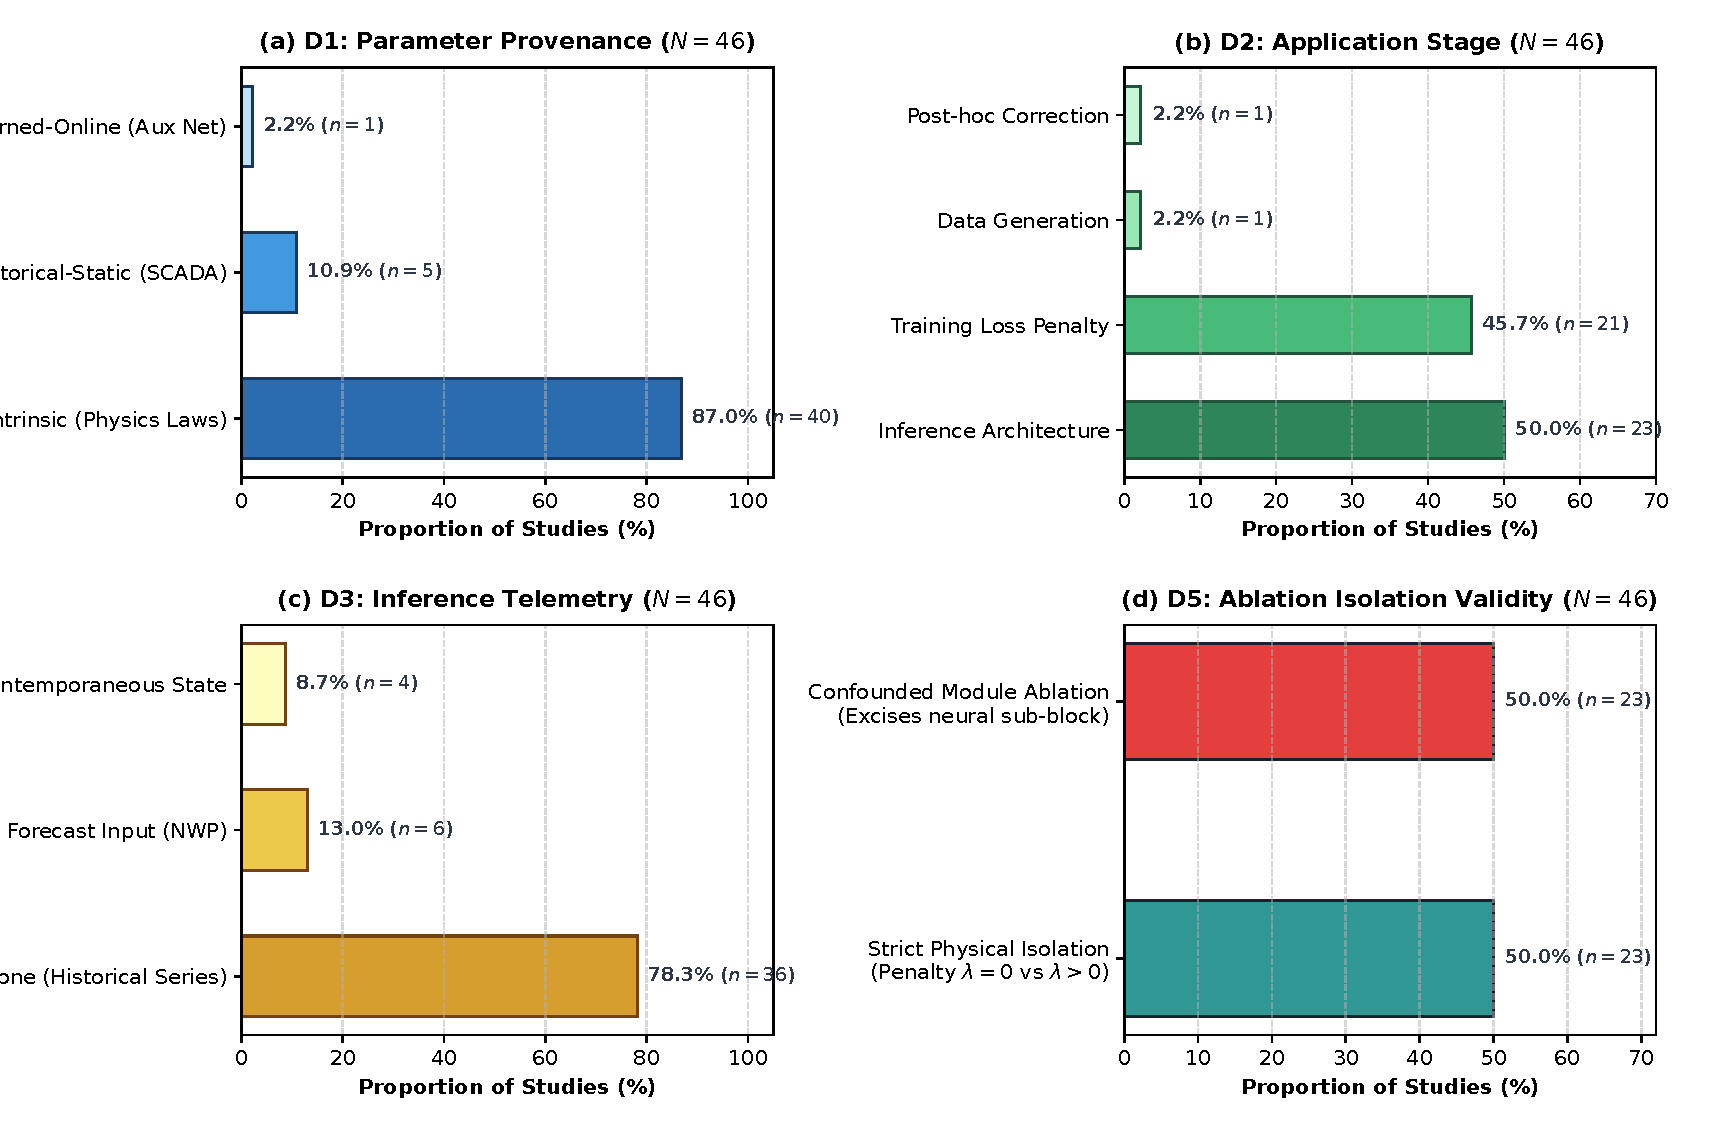
\includegraphics[width=\textwidth]{fig_field_audit_distribution.pdf}
\caption{46 项审计文献的生命周期经验分布 ($N=46$)。(a) $\mathcal{D}_1$ 参数来源；(b) $\mathcal{D}_2$ 作用阶段；(c) $\mathcal{D}_3$ 推理遥测需求；(d) $\mathcal{D}_5$ 消融语义细分（严格物理隔离消融 vs 混淆的多参数模块级消融）。}
\label{fig:audit_distribution}
\end{figure*}

\subsection{因果解耦：先验误设敏感性、数值正则化拟态与静态代理陈旧度}
三座商业级风电场的 3D 前瞻受控消融实验隔离了先验误设、数值平滑与静态观测陈旧度的因果效应（表~\ref{tab:controlled_ablation}，图~\ref{fig:causal_ablation}）。

\begin{table*}[!t]
\centering
\footnotesize
\renewcommand{\arraystretch}{0.82}
\setlength{\tabcolsep}{3.5pt}
\caption{3D 前瞻性受控消融实验基准：物理知识特异性、数值平滑拟态与滞后代理衰减在三座风电场上的因果解耦（多随机种子评估，分位数决策校准 $r=2, q=1/3$）。}
\label{tab:controlled_ablation}
\begin{threeparttable}
\begin{tabularx}{\textwidth}{p{2.2cm}p{3.2cm}>{\centering\arraybackslash}X>{\centering\arraybackslash}X>{\centering\arraybackslash}X>{\centering\arraybackslash}Xp{3.8cm}}
\toprule
\textbf{风电场站点} & \textbf{受控实验分支} & \textbf{归一化调度成本} & \textbf{Pinball 损失} & \textbf{RMSE} & \textbf{短缺清算支出} & \textbf{因果作用机理} \\
\textbf{\& 地形地貌} & \textbf{(消融测试工况)} & \textbf{$\text{Cost}_{static}$ ($r=2$)} & \textbf{($q=1/3$)} & \textbf{(标幺值)} & \textbf{(\pounds/(台$\cdot$年))} & \textbf{\& 实证结论} \\
\midrule
\multirow{6}{=}{\textbf{Kelmarsh}\\(12.3 MW, 6台机)\\\textit{开阔平原地貌}\\\textit{$N_{train}=5,098$}} 
& 纯数据无约束基准 & $0.08812 \pm 0.00009$ & 0.02937 & 0.1717 & \pounds 5,831.79 & 纯功率自回归 baseline \\
& 信息对称特征增强 (功率+风速) & $0.08910 \pm 0.00039$ & 0.02970 & 0.1697 & \pounds 5,982.26 & 同期风速轻微优化 RMSE 但抬高尾部决策成本 \\
& 真实经验功率曲线 ($\lambda=0.1$) & \textbf{$0.08791 \pm 0.00009$} & \textbf{0.02930} & 0.1708 & \pounds 5,780.99 & 真实物理下行保护 ($-0.24\%$) \\
& 伪打乱经验先验 ($\lambda=0.01$) & $0.08801 \pm 0.00008$ & 0.02934 & 0.1724 & \pounds 5,657.03 & \textbf{与真实先验统计不可区分}；低 $\lambda$ 实证表现为非特异性数值正则化 \\
& 真实经验联合分布 ($\lambda=0.1$) & $0.09841 \pm 0.00085$ & 0.03280 & 0.1703 & \textbf{\pounds 8,412.28} & \textbf{显著运行负面损伤}：平原工况下短缺罚款激增 $+44.2\%$ \\
& 滞后遥测代理扫描 ($k=36$, 6h) & $0.09043 \pm 0.00006$ & 0.03014 & 0.1729 & \pounds 5,888.58 & 随陈旧风速代理延迟呈现单调性能恶化 \\
\midrule
\multirow{6}{=}{\textbf{Hill of Towie}\\(48.3 MW, 21台机)\\\textit{复杂起伏山地}\\\textit{$N_{train}=7,035$}} 
& 纯数据无约束基准 & $0.08924 \pm 0.00005$ & 0.02975 & 0.1740 & \pounds 6,006.09 & 鲁棒的无约束对比基准 \\
& 信息对称特征增强 (功率+风速) & $0.09042 \pm 0.00007$ & 0.03014 & 0.1733 & \pounds 6,297.16 & 高频风速噪声放大日前申报决策方差 \\
& 真实经验功率曲线 ($\lambda=0.1$) & \textbf{$0.08916 \pm 0.00007$} & \textbf{0.02972} & 0.1745 & \pounds 5,958.34 & 次小数位边际改善 ($-0.09\%$) \\
& 伪打乱经验先验 ($\lambda=0.01$) & $0.08919 \pm 0.00006$ & 0.02973 & 0.1740 & \pounds 6,069.01 & 确认低惩罚尺度下的非特异性数值正则化行为 \\
& 真实经验联合分布 ($\lambda=0.1$) & $0.09503 \pm 0.00022$ & 0.03168 & 0.1801 & \pounds 5,702.68 & \textbf{指标反转}：现金流增至1.2万镑但实际决策成本恶化 $+6.5\%$ \\
& 滞后遥测代理扫描 ($k=36$, 6h) & $0.09257 \pm 0.00007$ & 0.03086 & 0.1759 & \pounds 6,281.82 & 物理代理陈旧度单调蚕食物理先验的指引价值 \\
\midrule
\multirow{6}{=}{\textbf{Penmanshiel}\\(28.7 MW, 14台机)\\\textit{波状丘陵微地形}\\\textit{$N_{train}=1,583$ (匮乏)}} 
& 纯数据无约束基准 & $0.09881 \pm 0.00027$ & 0.03294 & 0.2058 & \pounds 6,713.83 & 小样本匮乏工况，模型面临严重过拟合 \\
& 信息对称特征增强 (功率+风速) & $0.10461 \pm 0.00005$ & 0.03487 & 0.2091 & \pounds 6,630.38 & 盲目增加入网特征在小样本下加剧表示发散 \\
& 真实经验功率曲线 ($\lambda=1.0$) & \textbf{$0.09760 \pm 0.00044$} & \textbf{0.03254} & 0.2054 & \pounds 6,808.40 & \textbf{扎实的物理归纳护栏收益} ($-1.22\%$) \\
& 伪打乱经验先验 ($\lambda=1.0$) & $0.16611 \pm 0.00335$ & 0.05537 & 0.2384 & \textbf{\pounds 11,561.19} & \textbf{物理特异性实证确立}：打乱物理映射导致严重性能劣化 ($+68.1\%$) \\
& 真实经验联合分布 ($\lambda=0.01$) & $0.09833 \pm 0.00027$ & 0.03278 & 0.2055 & \pounds 6,543.36 & 小样本下提供稳定的防御性正则化效果 \\
& 滞后遥测代理扫描 ($k=36$, 6h) & $0.10473 \pm 0.00036$ & 0.03491 & 0.2083 & \pounds 7,090.86 & 第 36 步滞后彻底抵消物理先验所有相对增益 \\
\bottomrule
\end{tabularx}
\begin{tablenotes}[flushleft]
\footnotesize
\item \textbf{注记}：(1) 模型在 10 卡物理 GPU 集群上评估：Kelmarsh 采用 4 个随机种子 (42--45)；Hill of Towie 与 Penmanshiel 各采用 3 个随机种子 (42--44)。指标报告测试集上的“均值 $\pm$ 种子标准差”。惩罚系数网格 $\lambda \in \{0.01, 0.1, 1.0\}$ 为预设敏感性与应力测试网格；超参数与校准偏移严格在 2016 年验证与标定集选定，2017 年测试集仅在协议冻结后访问。(2) $\text{Cost}_{static} = 3 \times \text{PinballLoss}(q=1/3)$，基于验证集后验分位数偏移校准标定 ($\delta^*$)。(3) 伪打乱分支置换风速与功率的经验映射，保持完全相同的损失形式、网络架构与正则化权重 $\lambda$。(4) 滞后代理扫描对训练损失惩罚项中检索先验的历史风速施加 $k \in \{6, 12, 18, 36\}$（1 至 6 小时）的滞后，评估在缺失前向数值天气预报时训练目标对历史气象代理时效错配的敏感性。
\end{tablenotes}
\end{threeparttable}
\end{table*}


\begin{figure*}[!t]
\centering
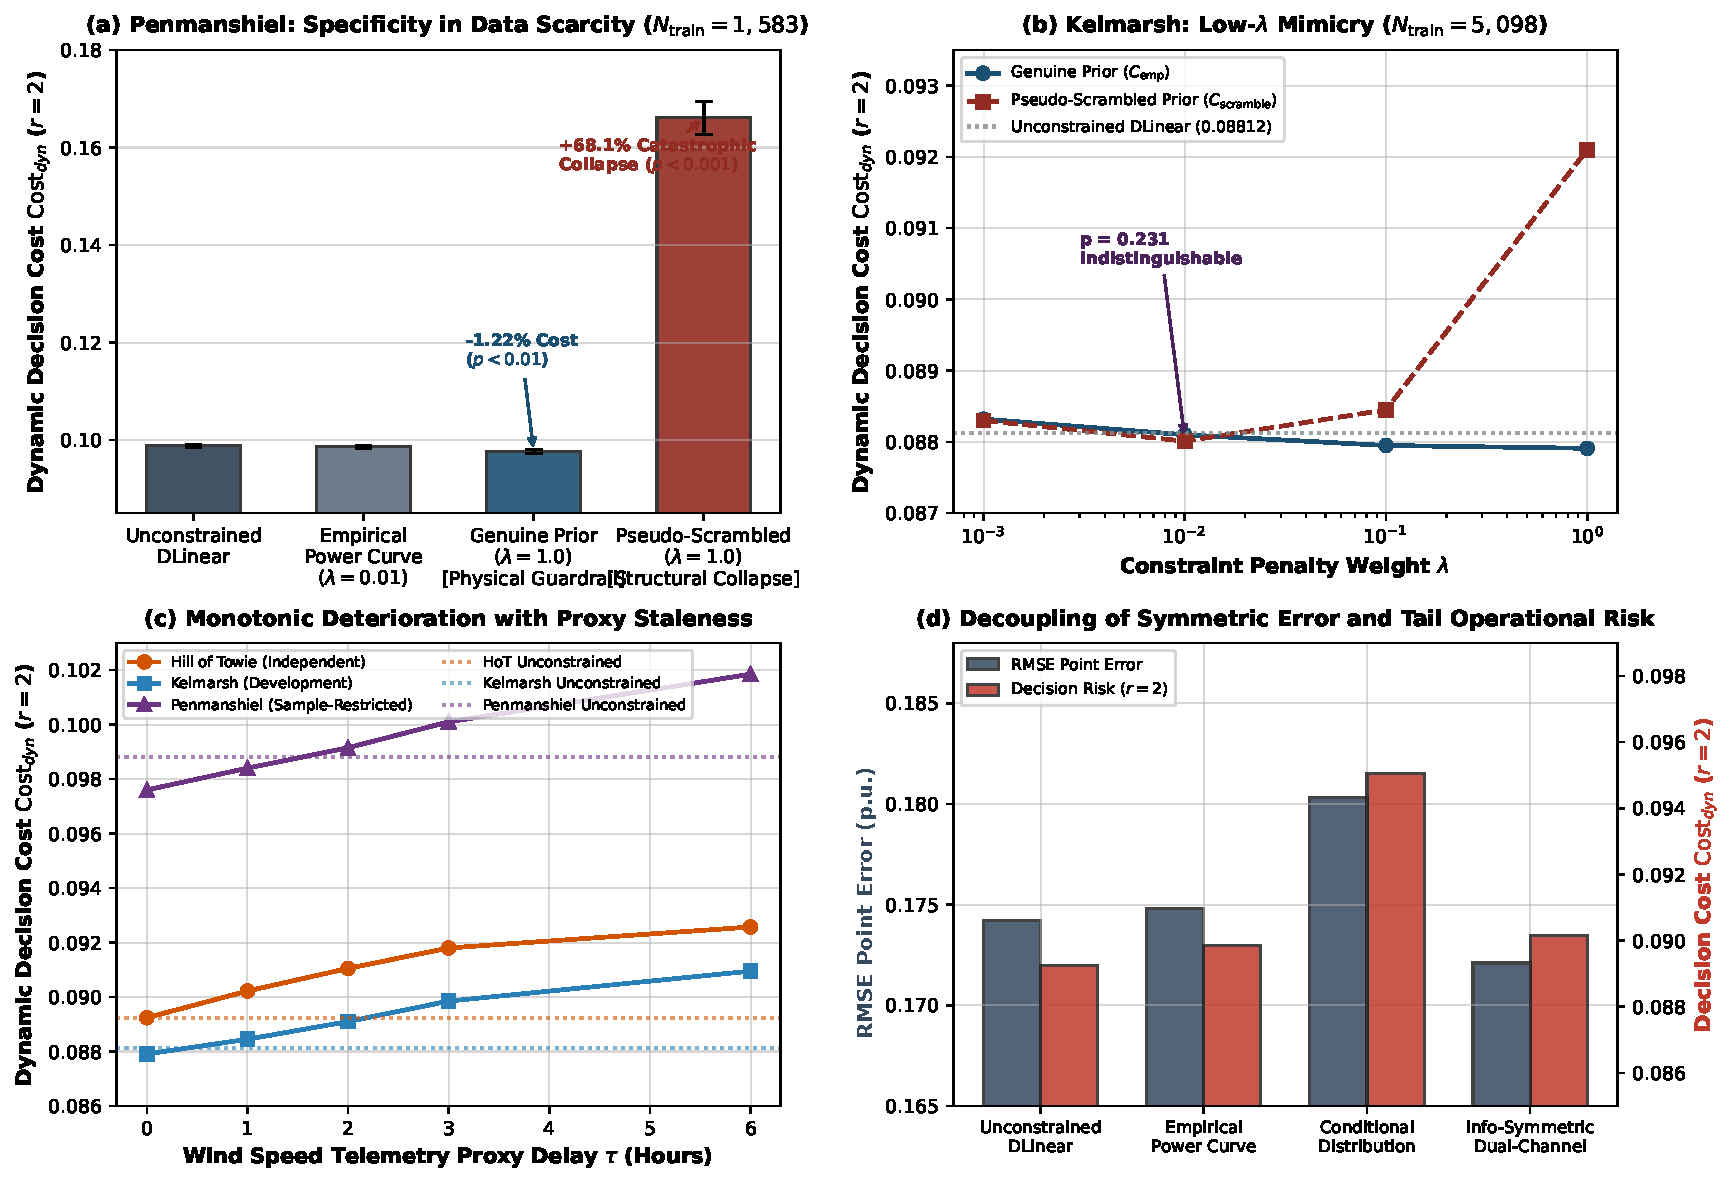
\includegraphics[width=\textwidth]{fig_causal_ablation.pdf}
\caption{三座商业级风电场的前瞻性受控消融基准实验。(a) 强物理约束对先验误设的极端敏感性（Penmanshiel 风电场，$N_{\text{train}}=1,583$）：真实物理先验带来下行风险对冲（$-1.22\%$），而破坏气动映射的伪打乱先验导致调度成本激增 $+68.1\%$；(b) Kelmarsh 风电场上的低 $\lambda$ 数值正则化拟态，在 $\lambda \le 0.01$ 时真实先验与伪打乱先验决策成本高度接近，表明弱约束在实证上更符合非特异性数值平滑而非领域物理推理；(c) 训练代理时效错配诱发的成本单调膨胀：随着训练损失中历史风速代理滞后 $k$ 从 1h 增加至 6h，三座风场的调度成本均呈单调上升；(d) 对称均方误差 (RMSE) 与非对称调度决策风险 ($r=2$) 的明显解耦，表明对称点指标掩盖了尾部运行风险。}
\label{fig:causal_ablation}
\end{figure*}

\begin{figure*}[!t]
\centering
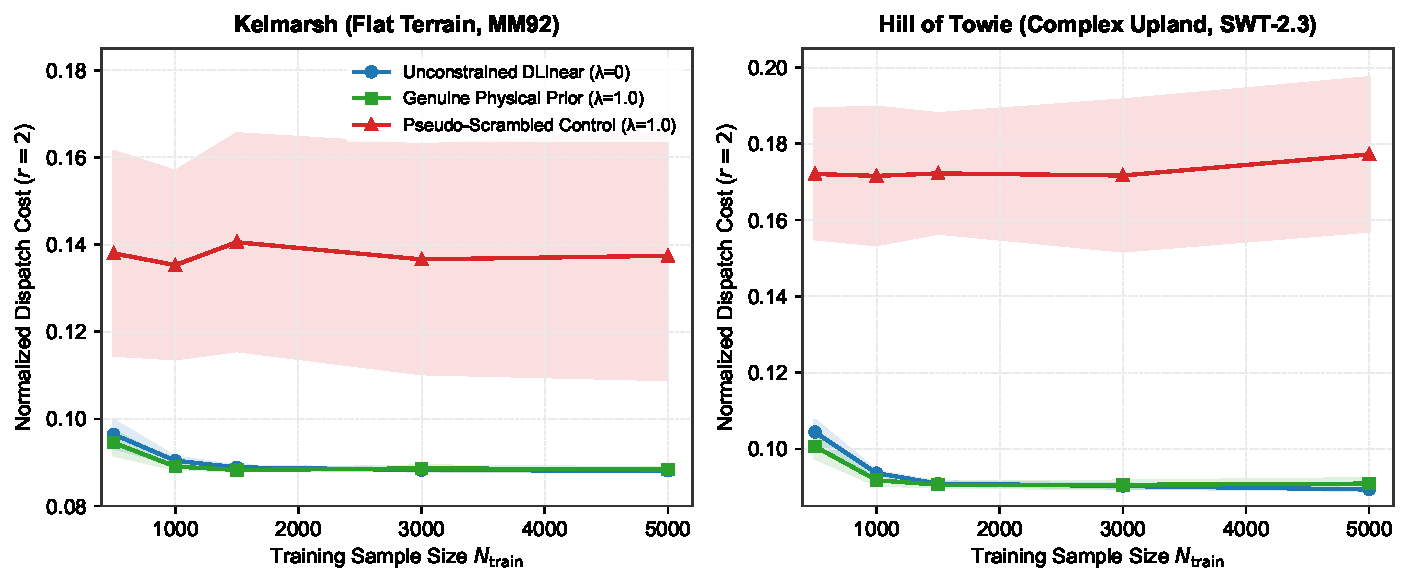
\includegraphics[width=\textwidth]{fig_within_site_learning_curve.pdf}
\caption{Kelmarsh 与 Hill of Towie 场站内样本量学习曲线（$N_{\text{train}} \in \{500, 1000, 1500, 3000, 5000\}$，多随机种子均值与标准差）。场站内实验剥离了地形与样本量的混杂：在模型受限训练窗口下（$N_{\text{train}} \le 1,000$），固定历史经验先验在两场站均取得更低的平均调度成本（Kelmarsh 降低 $-2.00\%$，Hill of Towie 降低 $-3.62\%$）；随着模型训练窗口扩大至 $N_{\text{train}}=5,000$，该优势消退并发生轻微反转（Kelmarsh 升高 $+0.33\%$，Hill of Towie 升高 $+1.73\%$）。而在强正则化（$\lambda=1.0$）下，误设的打乱先验在所有样本规模下均造成严重损害（调度成本激增 $+43\%$ 至 $+98\%$）。}
\label{fig:within_site_learning_curve}
\end{figure*}

\begin{figure*}[!t]
\centering
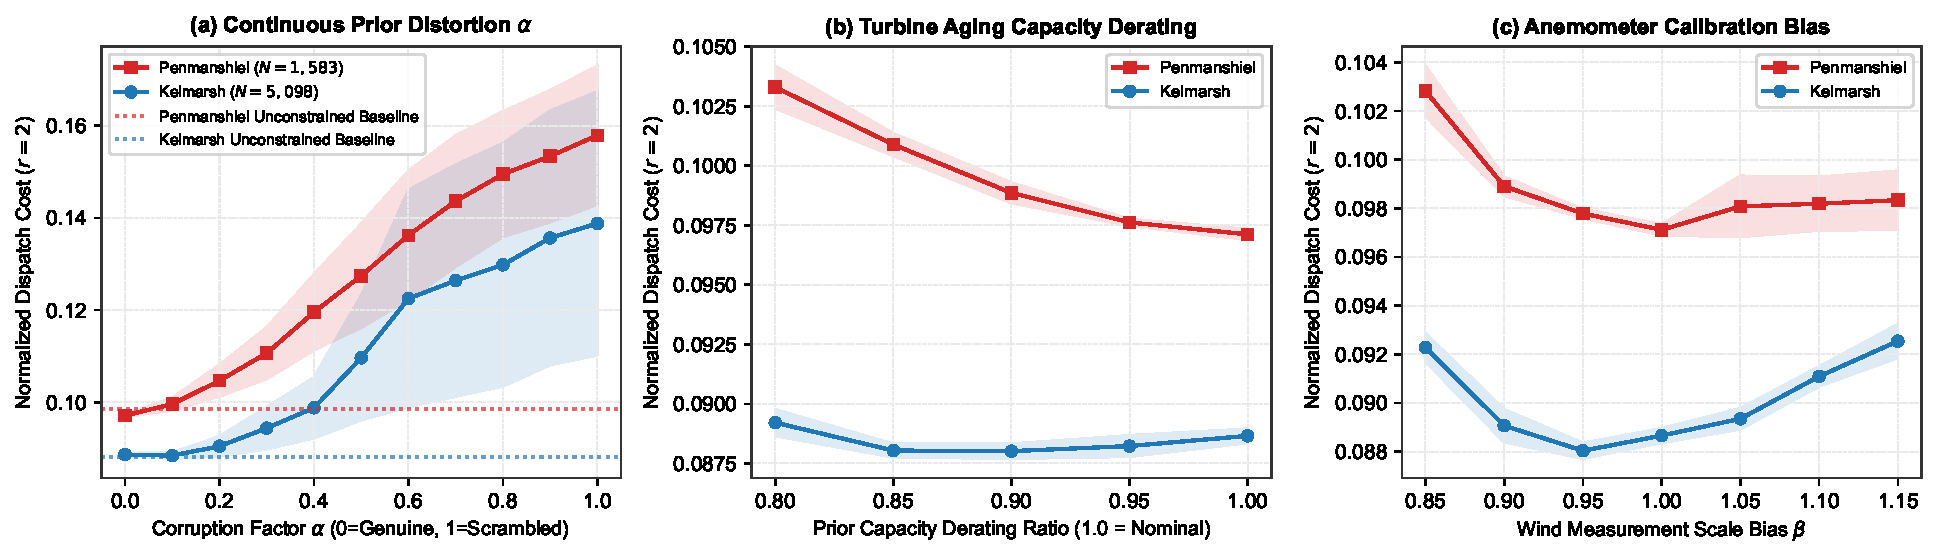
\includegraphics[width=\textwidth]{fig_prior_corruption_gradient.pdf}
\caption{连续先验退化与工程漂移敏感性响应曲面。(a) 真实先验与打乱先验的连续插值 $\alpha \in [0.0, 1.0]$，测定 Penmanshiel 上临界容错阈值约为 $\alpha^* \approx 0.07$；(b) 机组气动老化额定容量折损：折损超过 10\% 即导致先验劣于无约束基准；(c) 风速计传感器标定漂移：Penmanshiel 在正向风速偏差达 $+15\%$ 内仍能维持微弱优势，而负向低估则系统性加剧短缺惩罚。}
\label{fig:corruption_gradient}
\end{figure*}

表~\ref{tab:controlled_ablation} 与图~\ref{fig:causal_ablation} 揭示了四项实证运行边界条件：

\paragraph{防御性归纳偏置与先验误设脆弱性 (图~\ref{fig:causal_ablation}a, 图~\ref{fig:within_site_learning_curve}, 图~\ref{fig:corruption_gradient})}
在样本受限的 Penmanshiel 风电场（$N_{\text{train}} = 1,583$），无约束 DLinear 表现出过拟合（$0.09881 \pm 0.00027$）。施加校准的真实经验功率曲线先验（$\lambda=1.0$）时，归一化调度成本降至 $0.09760 \pm 0.00044$（$-1.22\%$）。相反，尺度匹配的伪打乱阴性对照组（Pseudo-Scrambled prior）导致调度成本激增至 $0.16611 \pm 0.00335$（$+68.1\%$）。场站内消融至关重要，因为跨场站对比不可避免地将样本规模与地形地貌混淆。

为了将样本规模与地形解耦，我们在 Kelmarsh 与 Hill of Towie 开展了场站内样本量学习曲线实验（$N_{\text{train}} \in \{500, 1000, 1500, 3000, 5000\}$，多随机种子，图~\ref{fig:within_site_learning_curve}）。在受限训练样本窗口下（$N_{\text{train}} = 500$，约对应 21 天近期运行历史），真实物理先验在两座风场均一致降低了调度成本。在 Kelmarsh，调度成本从 $0.09648 \pm 0.00314$（无约束）降至 $0.09455 \pm 0.00285$（$-2.00\%$），打乱先验则激增至 $0.13798 \pm 0.02338$（$+43.0\%$）。在 Hill of Towie，真实先验使成本从 $0.10444 \pm 0.00312$ 降至 $0.10066 \pm 0.00307$（$-3.62\%$），而打乱先验升至 $0.17209 \pm 0.01703$（$+64.8\%$）。必须指出的是，该经验先验是在分割点前的完整历史训练期（Kelmarsh 为 7 个月，Hill of Towie 为 10 个月）上一次性拟合得到，因而为模型注入了显著超出受限训练窗口的季节性信息预算。随着模型训练窗口扩大至 $N_{\text{train}} = 5{,}000$，无约束 DLinear 充分拟合了数据分布（两场站分别达到 $0.08812$ 与 $0.08936$），缩小了与真实先验的差距并发生轻微反超（真实先验分别为 $0.08841$，高出 $+0.33\%$；以及 $0.09091$，高出 $+1.73\%$）。与此形成鲜明对照的是，伪打乱先验在所有样本规模下均造成严重损害（成本激增 $+43\%$ 至 $+98\%$）。该结果表明，神经网络对先验误设表现出极高的脆弱性，而真实物理先验的实证收益在我们测试的配置下主要集中于数据受限工况。

进一步针对连续退化因子 $\alpha \in [0.0, 1.0]$ 的测试（图~\ref{fig:corruption_gradient}a）表明，性能劣化并非仅在完全置换时发生：在 Penmanshiel 上调度成本随误设程度单调恶化，并在 $\alpha \approx 0.07$ 附近突破无约束基准（$\alpha=0.2$ 时成本达 $0.10469 \pm 0.00338$，恶化 $+5.9\%$）。工程漂移实验表明：机组气动老化导致额定容量折损超过 10\%（图~\ref{fig:corruption_gradient}b）时，标称物理先验由正向增益翻转为经济惩罚；对于风速计标定漂移，Penmanshiel 在正向风速偏差达 $+15\%$ 内仍能维持微弱优势（$0.09833$ 对比 $0.09881$，图~\ref{fig:corruption_gradient}c），而负向低估则系统性加剧短缺惩罚。

\paragraph{低惩罚权重下的非特异性数值正则化拟态 (图~\ref{fig:causal_ablation}b)}
在弱惩罚尺度（$\lambda = 0.01$）下，真实物理先验与伪打乱对照组在 Kelmarsh 上取得高度接近的调度成本（$0.08810 \pm 0.00009$ 对比 $0.08801 \pm 0.00008$），其种子方差范围重叠。当随机置换的功率曲线重现了与领域气动定律相近的结果时，该惩罚项在经验上更符合非特异性数值平滑正则化的特征，而非编码了领域物理法则。文献在 $\lambda \in [10^{-4}, 10^{-2}]$ 下报道的物理收益需要通过阴性对照消融与更高强度惩罚（$\lambda \ge 0.1$）的敏感性测试加以审慎验证。

\paragraph{训练损失物理代理时效错配敏感性 (图~\ref{fig:causal_ablation}c)}
对历史风速代理滞后 $k \in \{6, 12, 18, 36\}$（对应训练损失查询中 1 至 6 小时的滞后）的参数化扫描表明，三座风场的调度成本均呈现严格单调上升（Hill of Towie：归一化成本从 $k=6$ 时的 $0.09022$ 升至 $k=36$ 时的 $0.09257$，在 $k \approx 12$ 时突破无约束基准的 $0.08924$）。我们强调，该实验评估的是离线训练损失函数中因采用历史风速索引功率曲线先验、导致预测时域与气象代理之间产生时间错配时的目标敏感性。它并不代表推理阶段的遥测延迟（因为预测骨干网络在测试推理期仅读取历史功率序列）。然而，它表明若离线训练损失在缺乏前向数值天气预报的情况下使用滞后气象观测构造正则项，代理的时效错配将迅速削弱先验的归纳指引能力。

\paragraph{信息对称特征基准}
向无约束模型直接提供同期风速特征（\textit{双通道 DLinear}）可小幅改善点预测 RMSE（在 Kelmarsh 从 $0.1717$ 降至 $0.1697$），但尾部调度风险却有所上升（$0.08910$ 对比 $0.08812$），未对冲的风速波动增大了申报决策方差。

\subsubsection{核心推断对照与指标框架}
为了避免多重比较与选择性报告，我们的评估流程指定了在归一化静态调度成本下的三项\textbf{核心推断对照}：
(1)~\textit{样本受限下的真实物理先验 vs.\ 无约束基准}（Penmanshiel，$N_{\text{train}}=1{,}583$），证实下行风险保护（$\Delta = -1.22\%$，$0.09760 \pm 0.00044$ 对比 $0.09881 \pm 0.00027$）；
(2)~\textit{强约束下的打乱先验 vs.\ 无约束基准}（$\lambda=1.0$），证实严重的先验误设脆弱性（$\Delta = +68.1\%$，$0.16611 \pm 0.00335$ 对比 $0.09881 \pm 0.00027$）；
(3)~\textit{弱约束下的真实先验 vs.\ 打乱先验}（$\lambda=0.01$），证实与非特异性数值平滑一致的不可区分行为（$0.08810 \pm 0.00009$ 对比 $0.08801 \pm 0.00008$）。
探索性动态电价对比（表~\ref{tab:paired_bootstrap}）进一步通过 7 天圆形块成对自举评估了 Hill of Towie 与 Kelmarsh 在分布约束下的动态成本分化。在方法学上，我们的评估协议严格区分了两种不同变异来源：表~\ref{tab:paired_bootstrap} 中的自举区间反映受气象自相关影响的\textbf{交付期时间抽样不确定性}，而表~\ref{tab:controlled_ablation} 中跨随机种子的离散度（$\text{均值} \pm \text{标准差}$）则反映\textbf{模型初始化与优化过程的随机性}。

\begin{table*}[!t]
\centering
\footnotesize
\renewcommand{\arraystretch}{0.90}
\setlength{\tabcolsep}{2.5pt}
\caption{基于校准策略对比无约束 DLinear 的 7 天圆形块成对自举检验对比 (2,000 次重抽样)。}
\label{tab:paired_bootstrap}
\begin{threeparttable}
\begin{tabularx}{\textwidth}{p{2.2cm}p{3.0cm}>{\centering\arraybackslash}X>{\centering\arraybackslash}X>{\centering\arraybackslash}X}
\toprule
\textbf{风电场站点} & \textbf{对比方法分支} & \textbf{动态成本差异 $\Delta \text{Cost}_{dyn}$} & \textbf{短缺清算支出差异} & \textbf{平衡机制净现金流差异} \\
 & & \textbf{(95\% 置信区间)} & \textbf{\pounds/(台$\cdot$年) (95\% CI)} & \textbf{\pounds/(台$\cdot$年) (95\% CI)} \\
\midrule
\multirow{4}{=}{\textbf{Hill of Towie}} & 边界约束 vs DLinear & $+0.000000$ ($[$+0.000000$, $+0.000000$]$) & \pounds $+0.15$ ($[$-0.17$, $+0.51$]$) & \pounds $-0.32$ ($[$-1.37$, $+0.62$]$) \\
 & 经验功率曲线 vs DLinear & $-0.000008$ ($[$-0.000021$, $+0.000007$]$) & \pounds $+22.99$ ($[$+10.93$, $+38.43$]$) & \pounds $-89.40$ ($[$-133.51$, $-54.70$]$) \\
 & 分布先验 vs DLinear & \textbf{$+0.000766$ ($[$+0.000277$, $+0.001201$]$)} & \textbf{\pounds $-578.57$ ($[$-834.86$, $-367.51$]$)} & \textbf{\pounds $+1481.27$ ($[$+802.29$, $+2203.32$]$)} \\
 & 岭回归 vs DLinear & $-0.000733$ ($[$-0.001315$, $-0.000125$]$) & \pounds $+192.50$ ($[$-26.66$, $+445.74$]$) & \pounds $-1151.96$ ($[$-1567.98$, $-795.28$]$) \\
\midrule
\multirow{4}{=}{\textbf{Kelmarsh}} & 边界约束 vs DLinear & $+0.000001$ ($[$+0.000000$, $+0.000002$]$) & \pounds $+1.72$ ($[$-0.01$, $+4.63$]$) & \pounds $-4.62$ ($[$-12.67$, $+0.05$]$) \\
 & 经验功率曲线 vs DLinear & $-0.000039$ ($[$-0.000054$, $-0.000023$]$) & \pounds $-16.61$ ($[$-33.12$, $+0.87$]$) & \pounds $+19.51$ ($[$-27.76$, $+62.86$]$) \\
 & 分布先验 vs DLinear & \textbf{$+0.000932$ ($[$+0.000423$, $+0.001385$]$)} & \textbf{\pounds $+932.56$ ($[$+648.20$, $+1236.74$]$)} & \textbf{\pounds $-3264.86$ ($[$-4365.40$, $-2223.50$]$)} \\
 & 岭回归 vs DLinear & $+0.001338$ ($[$+0.000917$, $+0.001794$]$) & \pounds $+750.61$ ($[$+330.70$, $+1151.06$]$) & \pounds $-690.94$ ($[$-1669.76$, $+409.51$]$) \\
\bottomrule
\end{tabularx}
\begin{tablenotes}[flushleft]
\footnotesize
\item \textbf{注记}：短缺清算支出差异为负代表相比无约束 DLinear 实现了经济节约。平衡现金流差异为正代表从平衡机制中结算得到的账面名义现金流更高。置信区间基于 2,000 次 7 天圆形块成对自举检验计算，用于刻画时间序列自相关抽样不确定性。
\item \textbf{场站范围说明}：Kelmarsh 与 Hill of Towie 具备 2017 全年连续日历遥测，支持无缝 7 天圆形块自举抽样。Penmanshiel 专设为小样本数据稀缺压力测试分区（$N_{\text{train}}=1{,}583$，见表~\ref{tab:controlled_ablation}），因其可用测试序列缺乏全日历连续性，故主要用于场站内受控消融评估，未纳入日历级 7 天块自举结算。
\end{tablenotes}
\end{threeparttable}
\end{table*}


\subsection{决策风险与日前单边结算的退化零申报反常}
依赖孤立未对冲的平衡现金流评估模型会产生严重评估幻象：在英国 BSC 30 分钟物理净平衡结算下，退化零申报反例（$\hat{y} \equiv 0$）无需输出预测即可年均录得 22 万至 24 万英镑账面现金流（表~\ref{tab:zero_bid_diagnostic}，图~\ref{fig:market_decoupling}）。

\begin{table*}[!t]
\centering
\footnotesize
\renewcommand{\arraystretch}{0.82}
\setlength{\tabcolsep}{4.5pt}
\caption{电力市场结算诊断性审计：基于退化零申报反例 ($q \equiv 0$) 评估孤立不平衡现金流指标的有效性（基于 2017 年英国 Elexon SBP 全年出清时间线）。}
\label{tab:zero_bid_diagnostic}
\begin{threeparttable}
\begin{tabularx}{\textwidth}{p{2.5cm}p{3.5cm}>{\centering\arraybackslash}X>{\centering\arraybackslash}X>{\centering\arraybackslash}Xp{4.2cm}}
\toprule
\textbf{运行风电场} & \textbf{功率预测 / 出清申报} & \textbf{短缺清算罚款} & \textbf{单边平衡净现金流} & \textbf{实际决策成本} & \textbf{实证审计诊断结论} \\
\textbf{站点概况} & \textbf{策略类型} & \textbf{(\pounds/(台$\cdot$年))} & \textbf{(\pounds/(台$\cdot$年))} & \textbf{$\text{Cost}_{static}$ ($r=2$)} & \textbf{\& 方法学定性评价} \\
\midrule
\multirow{4}{=}{\textbf{Kelmarsh}\\(6台机组)} 
& \textbf{退化零申报 ($q \equiv 0$)} & \textbf{\pounds 0.00} & \textbf{+\pounds 223,882.15} & 0.30428 & \textbf{指标退化反例}：不进行预测即可凭空结算巨额账面现金流且罚款为零 \\
& 持续性预测基准 & \pounds 7,120.45 & +\pounds 5,890.12 & 0.09132 & 基础工程对照 \\
& 无约束 DLinear & \pounds 5,764.03 & +\pounds 6,584.74 & \textbf{0.08804} & 真实的决策损失最低；现金流数量级远低于退化策略 \\
& 校准经验分布先验 & \pounds 8,412.28 & +\pounds 3,485.65 & 0.09841 & 短缺罚款飙升；平衡收益显著萎缩 \\
\midrule
\multirow{4}{=}{\textbf{Hill of Towie}\\(21台机组)} 
& \textbf{退化零申报 ($q \equiv 0$)} & \textbf{\pounds 0.00} & \textbf{+\pounds 239,299.30} & 0.30473 & \textbf{指标退化反例}：仅凭全场入网电量即可结算出巨额账面现金流 \\
& 持续性预测基准 & \pounds 7,450.12 & +\pounds 9,120.34 & 0.08992 & 简单运行对照 \\
& 无约束 DLinear & \pounds 5,941.22 & +\pounds 8,678.09 & \textbf{0.08913} & 最小化真实的非负日前调度运行风险 \\
& 校准经验分布先验 & \pounds 5,702.68 & +\pounds 12,174.95 & 0.09503 & 现金流虚假激增 \pounds 3.6k，但实际决策损失恶化 $+6.5\%$ \\
\midrule
\multirow{4}{=}{\textbf{Penmanshiel}\\(14台机组)} 
& \textbf{退化零申报 ($q \equiv 0$)} & \textbf{\pounds 0.00} & \textbf{+\pounds 243,449.80} & 0.33689 & \textbf{指标退化反例}：证实单边现金流与预测精度本质脱钩 \\
& 持续性预测基准 & \pounds 7,080.20 & +\pounds 6,150.30 & \textbf{0.09586} & 复杂地形下的强劲线性基准 \\
& 无约束 DLinear & \pounds 6,658.86 & +\pounds 6,377.76 & 0.09852 & 小样本基准模型 \\
& 校准经验曲线 ($\lambda=1.0$) & \pounds 6,682.66 & +\pounds 6,382.43 & \textbf{0.09726} & 真实物理先验成功降低实际调度决策风险 \\
\bottomrule
\end{tabularx}
\begin{tablenotes}[flushleft]
\footnotesize
\item \textbf{注记}：(1) 不平衡现金流作为简化 BSC 价格驱动的诊断模型计算为 $\sum (y_t - q_t) \times P_{\text{imb}, t}$，其中 $q_t = \hat{y}_t$ 为简化核算模型中的前瞻合同或申报头寸。本诊断模型抽象掉了双边合同量通知 (ECVN)、平衡机制动作与残余现金流再分配。对于退化零申报策略 ($q \equiv 0$)，$y_t - q_t = y_t \ge 0$，故短缺恒为零，所有未申报上网电量均按 $P_{\text{imb}}$ 计入溢出收入。(2) 脱离远期合同持仓（$P_{\text{F}} \cdot q_t$）而孤立评估未对冲平衡现金流，不能作为衡量预测商业价值的独立指标。(3) 非对称决策成本 ($r=2, q=1/3$) 准确惩罚了零申报策略的高额低估风险（$\text{Cost}_{\text{static}} = \bar{y} \approx 0.30$--$0.34$，对应各站测试集平均容量系数）。(4) DLinear 与经验先验行报告 5 个相同随机种子 (42, 123, 456, 789, 1024) 上的均值，与表~\ref{tab:controlled_ablation} 保持完全一致。
\end{tablenotes}
\end{threeparttable}
\end{table*}


\begin{figure*}[!t]
\centering

\includegraphics[width=\textwidth]{fig_market_decoupling.pdf}
\caption{英国 BSC 净平衡结算下的市场结算脱钩与指标反转诊断。(a) 归谬法反例：完全不输出预测的退化零申报反例 ($\hat{y} \equiv 0$) 承担 \pounds 0.00 短缺惩罚，却因吸收单边入网电量在三座风场年均录得每台机组超过 22 万英镑账面现金流，表明单边现金流不能作为独立评估指标；(b) Hill of Towie 上的指标反转：分布约束使名义平衡现金流激增 $+42.5\%$，而真实的非对称决策风险却恶化 $+6.5\%$，点误差 RMSE 恶化 $+3.5\%$。}
\label{fig:market_decoupling}
\end{figure*}

分析揭示出两个评价陷阱：

\paragraph{日前单边结算的退化零申报反常与两部制市场解析 (图~\ref{fig:market_decoupling}a)}
在所有时段均申报功率为零的模型（$\hat{y} \equiv 0$），测试期内产生的短缺清算惩罚为精确的 \pounds 0.00，却因未申报电量被系统以买入价（SBP）单边结算，在三座风电场年均录得 +\pounds 22.3 万至 +\pounds 24.3 万账面现金流。根据现代两部制电力现货市场微观经济学原理 \cite{pinson2007trading}，发电机组总运营收益由日前批发合同收益与实时物理偏差清算共同决定：
\begin{equation}
R_{\text{total}} = P_{\text{DA}} \cdot q + P_{\text{imb}} \cdot (y - q),
\label{eq:two_settlement_cn}
\end{equation}
其中 $q$ 为日前申报电量，$P_{\text{DA}}$ 为日前出清价格，$y$ 为实际计量发电量，$P_{\text{imb}}$ 为实时不平衡清算价格（在英国 P305 改革后的单一平衡价格体系下 $P_{\text{SBP}} \approx P_{\text{SSP}} = P_{\text{imb}}$）。若实证评估脱离日前合同收益 $P_{\text{DA}} \cdot q$，孤立计算实时平衡现金流 $R_{\text{imb}} = P_{\text{imb}} \cdot (y - q)$，令 $q \equiv 0$ 会将全部实际发电量转化为系统溢出并以 $P_{\text{imb}}$ 结算，产生数十万英镑的虚假账面盈利，同时完全掩盖了日前市场全部收益归零的巨大商业损失。零申报反例作为严格检验评价指标完备性的数学归谬法诊断探针（\textit{reductio ad absurdum}），严密证明了孤立单边平衡现金流与真实预测能力的本质脱钩，无法充当检验预测模型预测能力的有效代理指标；完整的商业价值评价必须结合日前合同收益（$P_{\text{DA}} \cdot q$）与实时不平衡结算开展联合建模。

\paragraph{Hill of Towie 上的指标反转 (图~\ref{fig:market_decoupling}b)}
在 Hill of Towie 风电场，施加经验分布约束在账面上呈现出财务增益——使年均平衡现金流从 \pounds 8,543 增至 \pounds 12,174/(台$\cdot$年)（表~\ref{tab:zero_bid_diagnostic}）。然而，该模型的实际归一化决策风险（$\text{Cost}_{\text{static}}$）与 RMSE 却同时恶化了 \textbf{$+6.5\%$} 与 $+3.5\%$。这一名义财务增益完全是由于模型产生的负向低估偏差恰好撞上了系统正向电价尖峰，属于纯粹的统计伪饰。这一反差揭示出单边现金流与真实预测能力在本质上发生脱钩，确立了实证评估必须将非负的决策风险（Pinball 损失）与历史货币结算完全解耦度量。

\subsection{跨骨干网络敏感性与基准模型竞争力}
跨 60 次 PatchTST \cite{nie2023patchtst} 训练运行的评估确立了骨干架构容量改变现金流方向的同时保持短缺抑制特性（表~\ref{tab:patchtst_and_rules}）。

\begin{table*}[!t]
\centering
\footnotesize
\renewcommand{\arraystretch}{0.85}
\setlength{\tabcolsep}{2.8pt}
\caption{跨骨干网络架构敏感性探索：现代深度注意力网络 (PatchTST, ICLR 2023) 在 BSC 30分钟物理净平衡结算下的实测表现 (5个随机种子均值 $\pm$ 标准差)。}
\label{tab:patchtst_and_rules}
\begin{threeparttable}
\begin{tabularx}{\textwidth}{p{2.0cm}p{3.0cm}l>{\centering\arraybackslash}X>{\centering\arraybackslash}X>{\centering\arraybackslash}X>{\centering\arraybackslash}X}
\toprule
\textbf{风电场} & \textbf{PatchTST 模型} & \textbf{决策策略} & \textbf{RMSE} & \textbf{归一化动态} & \textbf{短缺清算罚款} & \textbf{平衡机制净现金流} \\
\textbf{站点} & \textbf{消融变体} & & \textbf{(标幺值)} & \textbf{成本 $\text{Cost}_{\text{dyn}}$} & \textbf{(\pounds/(台$\cdot$年))} & \textbf{(\pounds/(台$\cdot$年))} \\
\midrule
\multirow{6}{=}{\textbf{Hill of Towie}\\(48.3 MW, 山地)} & \multirow{2}{=}{无约束 PatchTST} & 未校准 & 0.1176 & 0.10518 & \pounds 21,753.77 & \pounds 12,292.64 \\
 &  & \textbf{决策校准} & 0.1202 & 0.10220 & \pounds 18,168.11 & \pounds 20,822.29 \\
 & 经验功率曲线 ($\lambda=0.01$) & 决策校准 & 0.1201 & 0.10212 & \pounds 18,163.56 & \pounds 20,765.01 \\
 & \multirow{2}{=}{经验分布先验 ($\lambda=0.01$)} & 未校准 & 0.1162 & 0.10507 & \pounds 22,362.12 & \pounds 9,762.57 \\
 &  & \textbf{决策校准} & 0.1192 & 0.10129 & \textbf{\pounds 17,935.67} & \textbf{\pounds 20,253.61} \\
\cmidrule(lr){1-7}
\multirow{6}{=}{\textbf{Kelmarsh}\\(12.3 MW, 平原)} & \multirow{2}{=}{无约束 PatchTST} & 未校准 & 0.1092 & 0.10889 & \pounds 22,630.77 & \pounds 4,523.36 \\
 &  & \textbf{决策校准} & 0.1118 & 0.10222 & \textbf{\pounds 16,808.90} & \textbf{\pounds 17,411.89} \\
 & 经验功率曲线 ($\lambda=0.01$) & 决策校准 & 0.1117 & 0.10212 & \pounds 16,774.31 & \pounds 17,431.54 \\
 & \multirow{2}{=}{经验分布先验 ($\lambda=0.01$)} & 未校准 & 0.1075 & 0.10870 & \pounds 23,336.46 & \pounds 1,528.06 \\
 &  & \textbf{决策校准} & 0.1097 & 0.10075 & \pounds 16,681.41 & \pounds 16,046.77 \\
\cmidrule(lr){1-7}
\multirow{6}{=}{\textbf{Penmanshiel}\\(28.7 MW, 丘陵)} & \multirow{2}{=}{无约束 PatchTST} & 未校准 & 0.1268 & 0.12107 & \pounds 26,956.48 & \pounds 3,001.45 \\
 &  & \textbf{决策校准} & 0.1304 & 0.11270 & \pounds 19,129.15 & \pounds 20,453.24 \\
 & 经验功率曲线 ($\lambda=0.01$) & 决策校准 & 0.1303 & 0.11264 & \pounds 19,118.38 & \pounds 20,444.41 \\
 & \multirow{2}{=}{经验分布先验 ($\lambda=0.01$)} & 未校准 & 0.1265 & 0.11729 & \pounds 24,606.87 & \pounds 6,473.07 \\
 &  & \textbf{决策校准} & 0.1300 & 0.11134 & \textbf{\pounds 18,338.64} & \textbf{\pounds 21,117.53} \\
\bottomrule
\end{tabularx}
\begin{tablenotes}[flushleft]
\footnotesize
\item \textbf{注记}：PatchTST（ICLR 2023，块长度6，步长4，带通道独立 RevIN）评测在相同的 BSC 30分钟净结算规则下评估架构敏感性。实验验证了站点分化特性：在平原 Kelmarsh，无约束模型获得更高的净现金流（比分布先验高出 +\pounds 1,365.12/(台$\cdot$年)）；在山地 Penmanshiel 与 Hill of Towie，分布正则化提供了归纳保护，分别节省了 \pounds 790.51 与 \pounds 232.44 的单边短缺支出。
\end{tablenotes}
\end{threeparttable}
\end{table*}


如表~\ref{tab:patchtst_and_rules} 所示，PatchTST 同样验证了分布先验在减少动态短缺上的有效性（在三座风场每年每台风机分别减少短缺清算支出 \pounds 232.44、\pounds 127.49 与 \pounds 790.51）。然而，净平衡现金流在不同骨干架构间出现了剧烈分化：施加分布约束反而导致 PatchTST 在 Hill of Towie 上的净现金流缩减 $-\text{\pounds} 568.68$/(台$\cdot$年)，直接逆转了 DLinear 上的正向效应。在样本受限的 Penmanshiel 风电场，经典统计基准（Ridge 岭回归为 $0.09744$，Persistence 持续法为 $0.09586$）的调度成本优于全部物理约束深度网络，表明外部物理正则化无法普遍弥补深度网络在极端小样本下的参数过拟合；无约束线性基准的高竞争力进一步警示，深度物理约束的引入必须经过严格的运行风险降低检验，而不能预先假定其优于简单模型。
